\documentclass[a4,12pt]{horizon-theme}
\usepackage{lipsum}
\usepackage{fontawesome5}
\usepackage{graphicx,url}
\usepackage{float}
\usepackage{amsmath}
\usepackage{booktabs}
\usepackage{makecell}
\usepackage{array}
\usepackage{multirow}
\usepackage{caption}
\usepackage{subcaption}
\usepackage{siunitx}
\usepackage{enumerate}
\usepackage{gensymb}
\usepackage{csvsimple}
\usepackage{tabularray}
\usepackage{stackengine}
\usepackage{xcolor, colortbl}
\usepackage[round]{natbib}
\usepackage{karnaugh-map}
\usepackage{stackengine}
% \usepackage{longtable}
\usepackage{threeparttable}

\strutlongstacks{T}


% Cover Config
% \configCover{<num. do exp.>}{<data>}{<título>}
\configCover{5}{12/05/2022}{Transmissor de Dados Assíncrono}


\begin{filecontents*}{tb_verdade_ff.csv}
clk,clr,Q3,Q2,Q1,Q0,D3,D2,D1,D0
-,0,0,0,0,0,0,0,0,1
$\uparrow$,1,0,0,0,0,0,0,0,1
$\uparrow$,1,0,0,0,1,0,0,1,0
$\uparrow$,1,0,0,1,0,0,0,1,1
$\uparrow$,1,0,0,1,1,0,1,0,0
$\uparrow$,1,0,1,0,0,0,1,0,1
$\uparrow$,1,0,1,0,1,0,1,1,0
$\uparrow$,1,0,1,1,0,0,1,1,1
$\uparrow$,1,0,1,1,1,1,0,0,0
$\uparrow$,1,1,0,0,0,1,0,0,1
$\uparrow$,1,1,0,0,1,1,0,1,0
$\uparrow$,1,1,0,1,0,0,0,0,0
$\uparrow$,1,1,0,1,1,-,-,-,-
$\uparrow$,1,1,1,0,0,-,-,-,-
$\uparrow$,1,1,1,0,1,-,-,-,-
$\uparrow$,1,1,1,1,0,-,-,-,-
$\uparrow$,1,1,1,1,1,-,-,-,-
\end{filecontents*}

\begin{filecontents*}{vcc1.csv}
pos,comp,vcc,gnd
sr1,74166,16,8
sr2,74166,16,8
c1,74163,16,8
p1,74280,14,7
ff1,7474,14,7
or1,7432,14,7
or2,7432,14,7
or3,7432,14,7
or4,7432,14,7
and1,7408,14,7
nand1,7400,14,7
nand2,7400,14,7
\end{filecontents*}

\begin{filecontents*}{tb_dep.csv}
clk,envia,reset, d_Qa,d_Qb,d_Qc,d_Qd, d_ff,d_pe,d_disable,d_preload, d_sr,Tx, Obs
$\uparrow$,$\uparrow$,1,    0,0,0,0,    1,0,1,1,    0,1,          $^1$
$\uparrow$,$\times$,1,      1,0,0,0,    1,1,1,1,    0,0,          $^2$
$\uparrow$,$\times$,1,      0,1,0,0,    1,1,1,1,    $d_0$,$d_0$,  $^3$
$\uparrow$,$\times$,1,      1,1,0,0,    1,1,1,1,    $d_1$,$d_1$,  $^4$
$\uparrow$,$\times$,1,      0,0,1,0,    1,1,1,1,    $d_2$,$d_2$,  $^5$
$\uparrow$,$\times$,1,      1,0,1,0,    1,1,1,1,    $d_3$,$d_3$,  $^6$
$\uparrow$,$\times$,1,      0,1,1,0,    1,1,1,1,    $d_4$,$d_4$,  $^7$
$\uparrow$,$\times$,1,      1,1,1,0,    1,1,1,1,    $d_5$,$d_5$,  $^8$
$\uparrow$,$\times$,1,      0,0,0,1,    1,1,1,1,    $d_6$,$d_6$,  $^9$
$\uparrow$,$\times$,1,      1,0,0,1,    1,1,1,1,    $p$,$p$,      $^{10}$
$\uparrow$,$\times$,1,      0,1,0,1,    0,1,0,0,    1,1,          $^{11}$
$\uparrow$,$\times$,1,      0,0,0,0,    0,0,1,1,    1,1,          $^{12}$
$\uparrow$,$\times$,1,      0,0,0,0,    0,0,1,1,    1,1,          $^{13}$
$\times$,$\times$,0,        $\times$,$\times$,$\times$,$\times$,    0,$\times$,1,0,    0,1,          $^{14}$
\end{filecontents*}


\begin{document}
\horizonCover

\horizonTitle


\section{Introdução} % R

A transmissão serial de dados de um sistema digital para outro é normalmente usada para reduzir o número de fios na linha de transmissão. Nesse tipo de comunicação é utilizada apenas dois fios, um de sinal GND e outro para a transmissão dos dados. Por exemplo, alguns periféricos do computador utilizam comunicação serial para se comunicarem com a placa mãe, tal qual o mouse e o teclado.

Nesse projeto será abordada apenas a comunicação serial assíncrona, na qual é transmitido um bit por vez, iniciando com um bit especial (bit Start) que tira a comunicação do repouso e indica a transmissão dos dados, e terminando com dois bits que indicam o fim da comunicação (bit Stop).

\section{Objetivos} % N
O objetivo deste experimento é projetar, simular, construir e testar um transmissor de dados assíncrono que transmita pacotes de dados de acordo com o protocolo RS232 e usando paridade ímpar.



\section{Planejamento} % N, R
\label{sec:plan}

\subsection{Diagrama de blocos}
\label{sec:blocos}
A Fig. \ref{fig:blocos} mostra o diagrama de blocos do circuito transmissor de dados assíncrono. Este circuito recebe os dados em paralelo e performa a serialização dos dados usando registradores de deslocamento. O circuito controlador implementa a lógica que liga/desliga o caregegamento/serialização do registradores de deslocamento para que apenas um pacote seja enviado após o sinal envia. E, como os dados precisam ser transmitidos de acordo com o padrão RS232, há ainda a necessidade de calcular o bit de paridade e colocar o sinal Tx no nível lógico '1' (Mark) quando em repouso. Isso é feito pelo bloco gerador de paridade e circuito combinatório, respectivamente. 

{\bf Importante:} O sinal reset é equivalente ao sinal ``limpa'' do enunciado.

\begin{figure}[!ht]
    \centering
    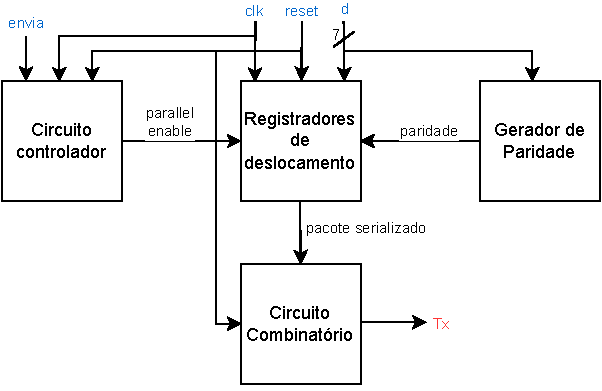
\includegraphics[width=0.87\textwidth]{blocos}
    \caption{Diagrama de blocos do circuito com entradas em azul e saída em vermelho}
    \label{fig:blocos}
\end{figure}

\subsection{Síntese do Circuito} % N, R
\label{sec:sintese}

Na síntese do circuito transmissor de dados assíncrono, a primeira decisão tomada foi a escolha do CI que realizaria a conversão dos dados paralelos em dados seriais, para isso, utilizou-se o CI 74166 que já faz essa conversão internamente necessitando apenas de entradas de controle para configurá-lo. Como o circuito 74166 só possui 8 entradas paralelas optou-se por expandi-lo através da utilização de dois CIs desse tipo. A ligação para essa expansão consiste simplesmente em ligar a saída "QH" de um deles na entrada serial ("SER") do outro. 

Para o controle desse "conversor paralelo serial" foi utilizado o contador módulo 11 projetado no experimento 4, porém com mais uma lógica, que no diagrama lógico tem o sinal "d\_pe" como seu resultado. Sabe-se, pelo datasheet, que o 74166 só carrega as entradas paralelas, na próxima borda de subida do clock, quando a sua entrada de controle "STLD" está em 0. E, para esses dados serem enviados serialmente pela saída "QH" é preciso que a entrada "STLD" esteja em 1. Portanto, essa lógica adicional implementada no contador nada mais é do que um resultado zero somente quando o contadador está em estado zero, ou seja, um OR de todas as saídas de estado do contador. Já o sinal "d\_disable" é o resultado da lógica que transforma o contador 74163, que naturalmente é um contador módulo 16, em um contador módulo 11. Esse sinal foi obitido através da negação da equação algébrica resultante do mapa de Karnaugh da Fig.\ref{fig:karnaugh_74163}
do apêndice.

Como a transmissão serial de dados assíncrona precisa seguir um protocolo de comunicação, precisamos colocar um bit que indica o início da trasmissão (o bit "Start") e dois bits que indicam o final (o bit "Stop"). Para isso, colocou-se a entrada "H" do primeiro 74166 em GND e as entradas "F" e "G" do segundo 74166 em VCC.

A fim de controlar os CIs 74166 e o contador para só iniciarem a transmissão dos dados quando o sinal "envia" for ativado, utilizou-se um flip-flop do CI 7474 com o próprio sinal envia na entrada de clock, e colocou-se a saída negada do flip-flop na entrada de controle "ENP" do contador, ou seja, o contador só começa a contágem e o 74166 só começa a transmissão dos dados quando o sinal envia é ativado.

Por fim, implementou-se a lógica que resulta no sinal de saída "Tx" pensando na padronização da comunicação para ficar em alta quando o transmissor está em repouso e, durante a transmissão, transmitir os dados sem interferência. Como pode ser visto no diagrama lógico da Fig \ref{fig:diagrama-logico}, essa lógica consiste em uma porta lógica OR ligada à saída do 74166 com a saída de uma porta NAND que tem como entradas o sinal "d\_pe" e o sinal "reset".

\newpage
\subsection{Diagrama Lógico}
\label{sec:diagrama-logico}

\begin{figure}[!ht]
    \centering
    \stackinset{r}{1pt}{t}{1pt}{\carimboA{Transmissor Assíncrono}}{%
        \stackinset{r}{1pt}{t}{67pt}{\carimboB{vcc1.csv}}{%
            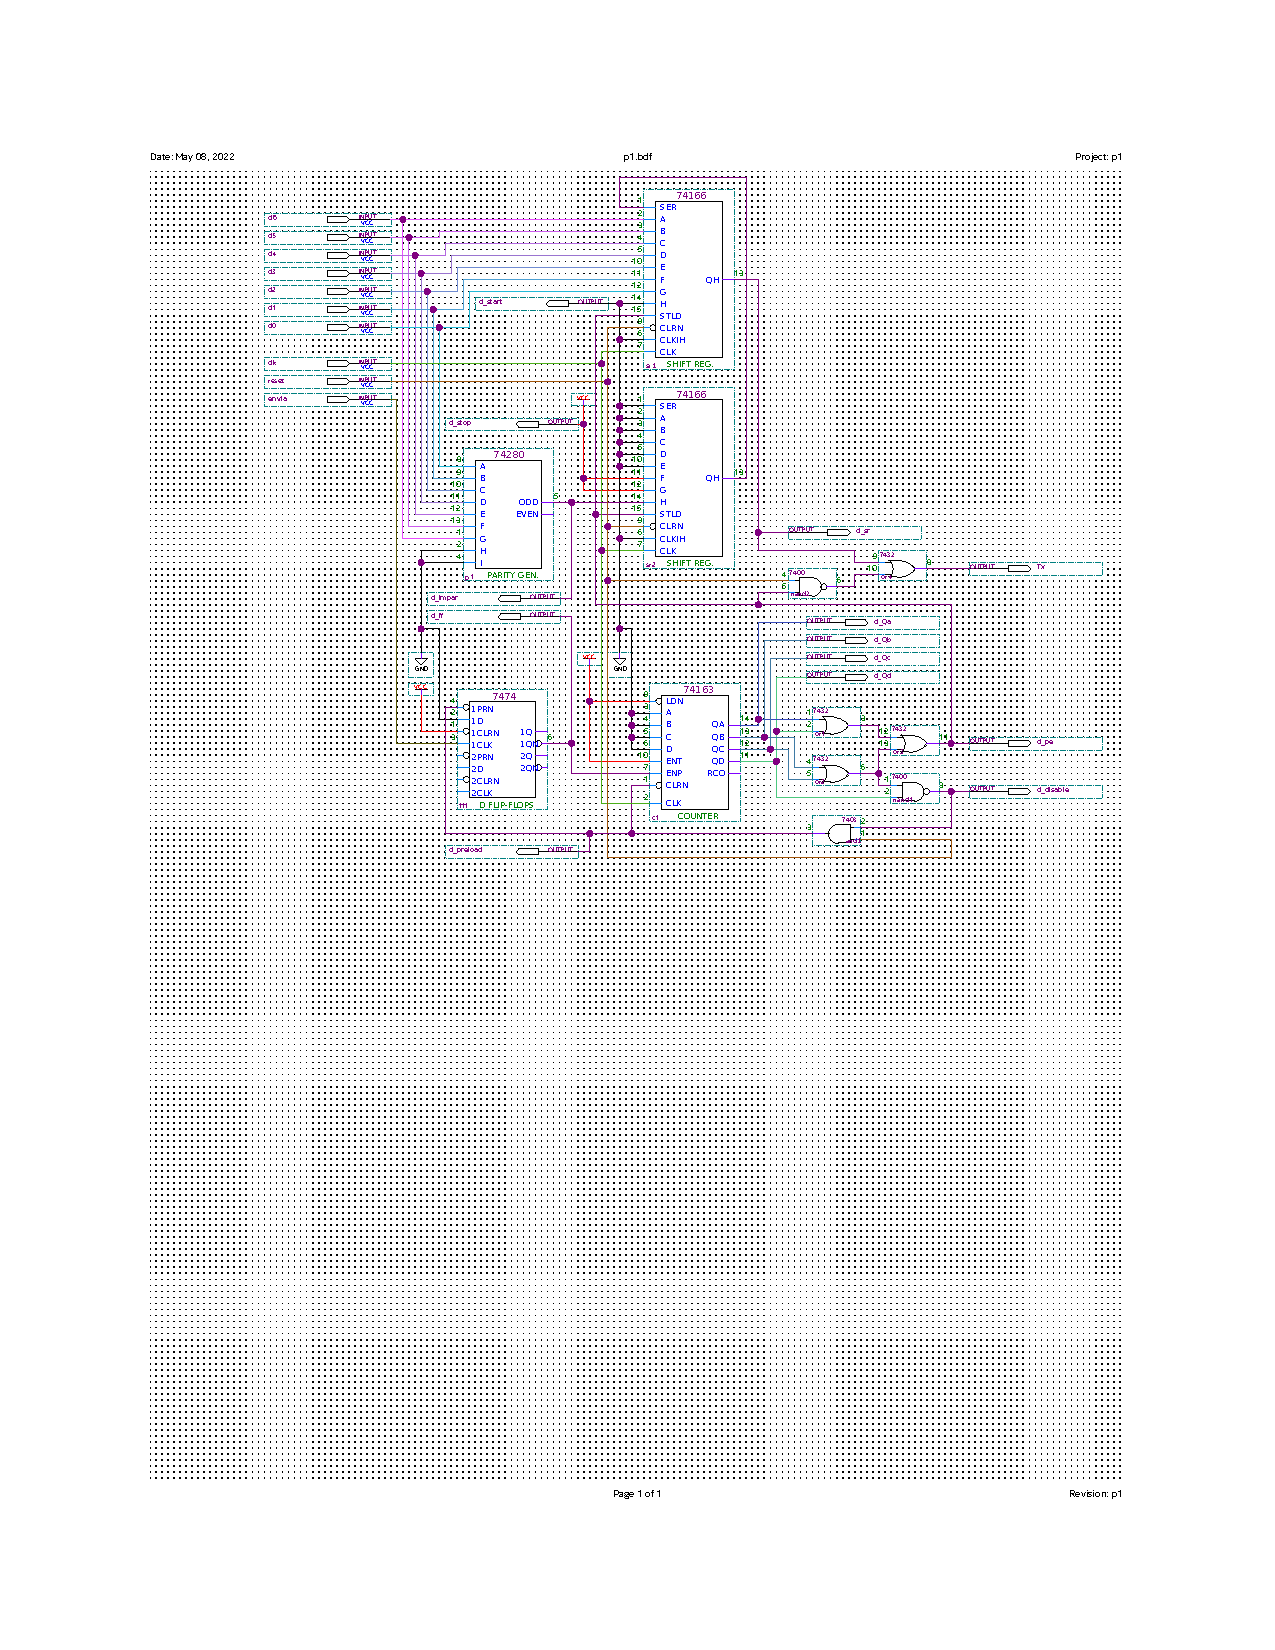
\includegraphics[width=\textwidth, trim={44mm, 133mm, 28mm, 29mm}, clip]{p1}%
        }%
    }
    \caption{Diagrama lógico do transmissor assíncrono.}
    \label{fig:diagrama-logico}
\end{figure}

A Fig. \ref{fig:diagrama-logico} mostra o diagrama lógico criado com o método de síntese especificado na Seção \ref{sec:sintese}. A disponibilidade dos componentes usados no diagrama foi conferida durante o OpenLab.


\subsection{Simulação}

\begin{figure}
    \centering
    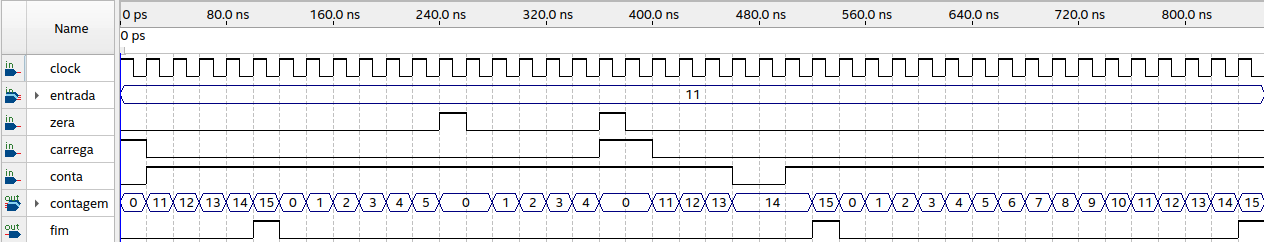
\includegraphics[width=\textwidth]{contador}
    \caption{Carta dos tempos do circuito contador}
    \label{fig:ct_contador}
\end{figure}

Quatro casos de teste foram elaborados para validar a lógica do circuito projetado. Cada caso de teste possui uma descrição em alto nível de um comportamento esperado do sistema. Essas descrições são, então, convertidas em estímulos dos sinais de entrada para criação da carta dos tempos, uma para cada caso de teste. A inspeção dessas cartas dos tempos diz se a resposta do circuito está coerente com a esperada. Esses casos de teste estão detalhados nos Apêndices \ref{ap:tc-1}, \ref{ap:tc-2}, \ref{ap:tc-3} e \ref{ap:tc-4}.

A análise de cada uma das cartas dos tempos (Figs. \ref{fig:tc1}, \ref{fig:tc2}, \ref{fig:tc3} e \ref{fig:tc4}) mostrou que o circuito projetado passou em todos os casos de teste.




\subsection{Levantamento dos materiais necessários}
\label{sec:materiais}

\begin{table}[!ht]
    \centering
    \caption{Unidades requeridas para cada CI}
    \label{tab:materiais}
    \doubleRuleSep
    \begin{tabular}{lllrr}
        \doubleTopRule
        Slot & Operação & CI & Un. Requeridas & Un. Disponíveis \\
        \midrule
        1 & Reg. Desl. & 74166 & 1 & 1\\
        2 & Reg. Desl. & 74166 & 1 & 1\\
        3 & Ger. Par. & 74280 & 1 & 1\\
        4 & Flip-Flop & 7474 & 1 & 2\\
        5 & Contador & 7463 & 1 & 1\\
        6 & And-2 & 7408 & 1 & 4\\
        7 & Or-2 & 7432 & 4 & 4\\
        8 & Nand-2 & 7400 & 2 & 4\\
        \doubleBottomRule
    \end{tabular}
\end{table}

Para garantir que o circuito projetado respeite as restrições de montagem, fizemos um levantamento dos recursos necessários para este circuito mostrado na Tabela \ref{tab:materiais}. Ela mostra a quantidade de unidades lógicas requeridas para cada CI utilizado. As especificações de cada CI foi obtido pelos respectivos \emph{datasheets}.



\subsection{Metodologia de montagem}
\label{sec:montagem}

A montagem será feita reduzindo o circuito em duas partes menores $\mathcal{P}_1$ e $\mathcal{P}_2$. Separamos essas partes de forma a ser possível depurá-las separadamente usando as cartas dos tempos e a tabela de depuração nos Apêndices \ref{ap:tc} e \ref{ap:tb-dep}, respectivamente. $\mathcal{P}_1$ é constituída pelos componentes c1, or1, or2, or3, nand1, and1 e ff1 do diagrama lógico (Fig. \ref{fig:diagrama-logico}) e $\mathcal{P}_2$ é constituída pelos componentes p1, sr1, sr2, nand2 e or4. Para otimizar o tempo de montagem, $\mathcal{P}_1$ e $\mathcal{P}_2$ serão montadas em paralelo. As entradas de $\mathcal{P}_1$ são \texttt{clk}, \texttt{reset} e \texttt{envia} e os sinais de depuração são \texttt{d\_Qa}, \texttt{d\_Qb}, \texttt{d\_Qc}, \texttt{d\_Qd}, \texttt{d\_preload}, \texttt{d\_ff}, \texttt{d\_disable} e \texttt{d\_pe}, sendo esse último uma das entrada de $\mathcal{P}_2$. Os sinais de entrada de $\mathcal{P}_2$ são os 7 bits de dados, clk e reset, com substituição do sinal \texttt{d\_pe} por VCC para simular esse sinal durante a transmissão, e os sinais depuração são \texttt{d\_impar}, \texttt{d\_sr} e a saída do circuito \texttt{Tx}.


\section{Resultados}

% A Fig. \ref{fig:onda} mostra o sinal gerado com a transmissão de um pacote de dados. Nela é possível identificar, da esquerda para direita, o sinal inicialmente em estado de repouso, o \texttt{start bit} (nível lógico 0), uma palavra de 7 bits $(1011001)_2$, que são os dados transmitidos, o bit de paridade, o \texttt{stop bit} (nível lógico 1), e, por fim, o estado de repouso novamente.

O circuito transmissor de dados foi montado conforme o diagrama lógico da Fig. \ref{fig:diagrama-logico} e testado conforme os casos de teste descritos nos Apêndices \ref{ap:tc} e \ref{ap:tb-dep}. Durante a montagem (Fig. \ref{fig:montagem}) foi notado um problema de Hazard no circuito causando um atraso no sinal \texttt{d\_preload}, sendo esse sinal substituído por uma chave. Por isso, o pacote não pode ser transmitido pelo TeraTerm da forma esperada. O pacote era transmitido corretamente apenas ao ligar o circuito.

\begin{figure}[!ht]
    \centering
    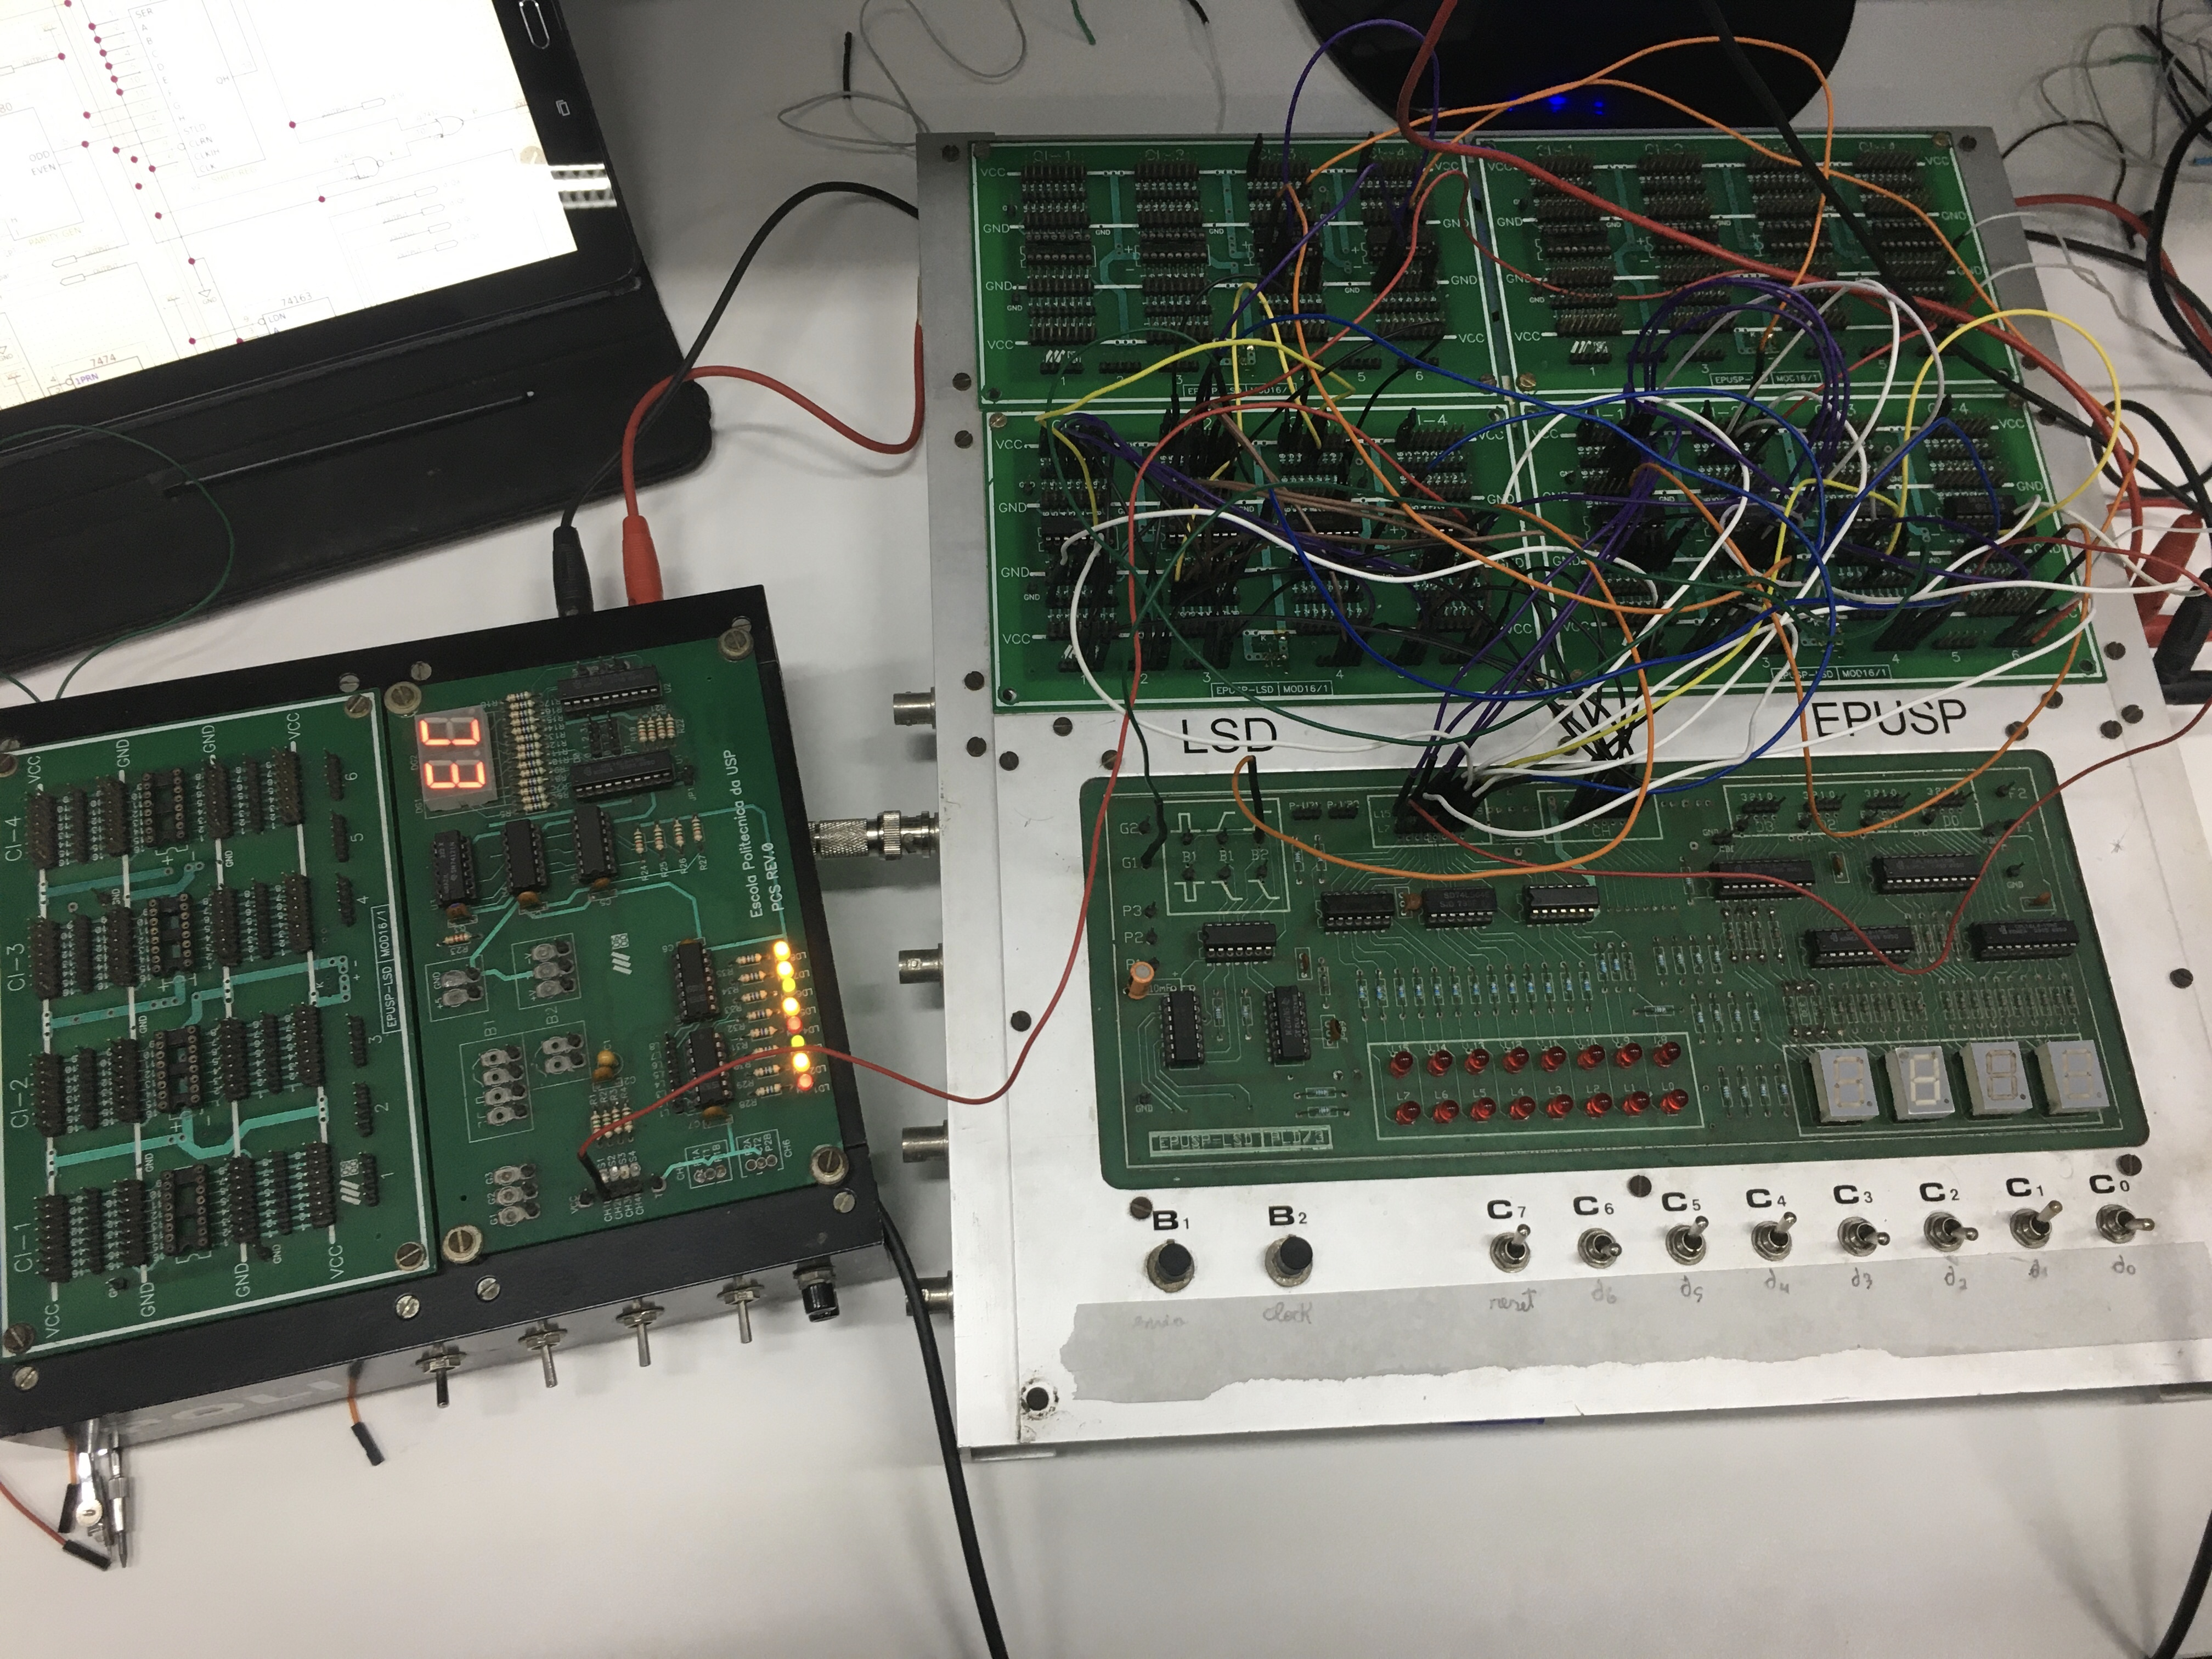
\includegraphics[width=0.6\textwidth]{montagem.jpeg}
    \caption{Montagem do circuito}
    \label{fig:montagem}
\end{figure}


\section{Conclusão}
Concluímos que, a partir do circuito lógico projetado, foi possível implementar um circuito na placa de montagem que cumpriu parcialmente com os requisitos. Houve a transmissão do caractere desejado, porém, para clocks de alta frequência, não era possível parar a transmissão manualmente.




\newpage

\appendix
\section*{Apêndice}
\renewcommand{\thesubsection}{\Alph{subsection}}

\subsection{Casos de Teste}
\label{ap:tc}

\subsubsection{Primeiro Caso de Teste}
\label{ap:tc-1}
{\bf Descrição do Caso de Teste:} O sinal \texttt{Tx} deve estar inicialmente em estado de repouso (nível lógico '1'). Assim que o sistema  receber o sinal \texttt{envia}, os dados paralelos devem ser carregados no próximo sinal de relógio. No clock de carregamento, o sinal \texttt{Tx} deve permanecer em estado de repouso e no sinal de relógio subsequente deve tranmitir apenas um pacote de dados e voltar imediatamente para o estado de repouso. O pacote deve ser consituído por um bit  \texttt{start} (nível lógico '0'), uma palavra com os 7 bits de dados, um bit de paridade ímpar e dois bits \texttt{stop} (nível lógico '1').

Esse é um caso de teste base e testa as características fundamentais do sistema.

\begin{figure}[!ht]
    \centering
    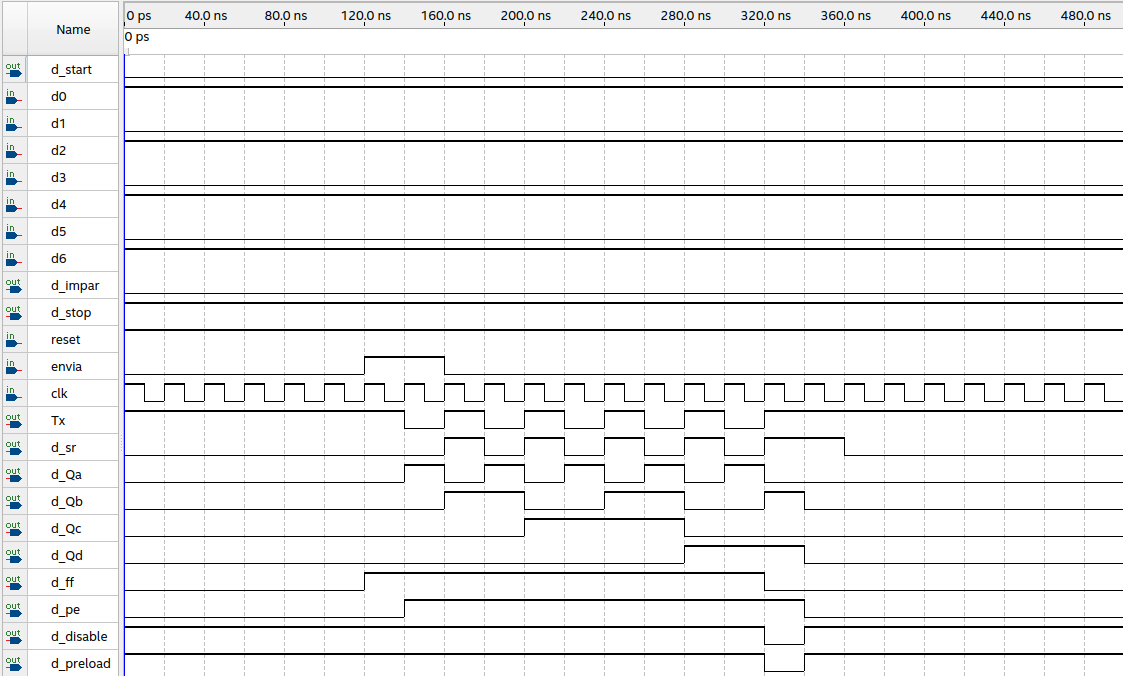
\includegraphics[width=\textwidth]{tc-1.png}
    \caption{Carta dos Tempos do primeiro caso de teste}
    \label{fig:tc1}
\end{figure}

\newpage
\subsubsection{Segundo Caso de Teste}
\label{ap:tc-2}
{\bf Descrição do Caso de Teste:} Assim que o sistema receber o sinal \texttt{reset} no nível lógico '0' ele deve interromper imediatamente a transmissão e o sinal \texttt{Tx} deve voltar imediatamente para o estado de repouso. O interrompimento da transmissão não deve influenciar na transmissão seguinte. Assim, no próximo sinal \texttt{envia}, o sistema deve carregar novamente os dados e transmitir o pacote com os novos valores de dados.

Esse caso de teste tem finalidade de identificar possíveis efeitos colaterais (e.g. iniciar transmissão seguinte com contador diferente de zero) nos registradores de deslocamento e nos estados do contador causados pelo sinal reset.
\begin{figure}[!ht]
    \centering
    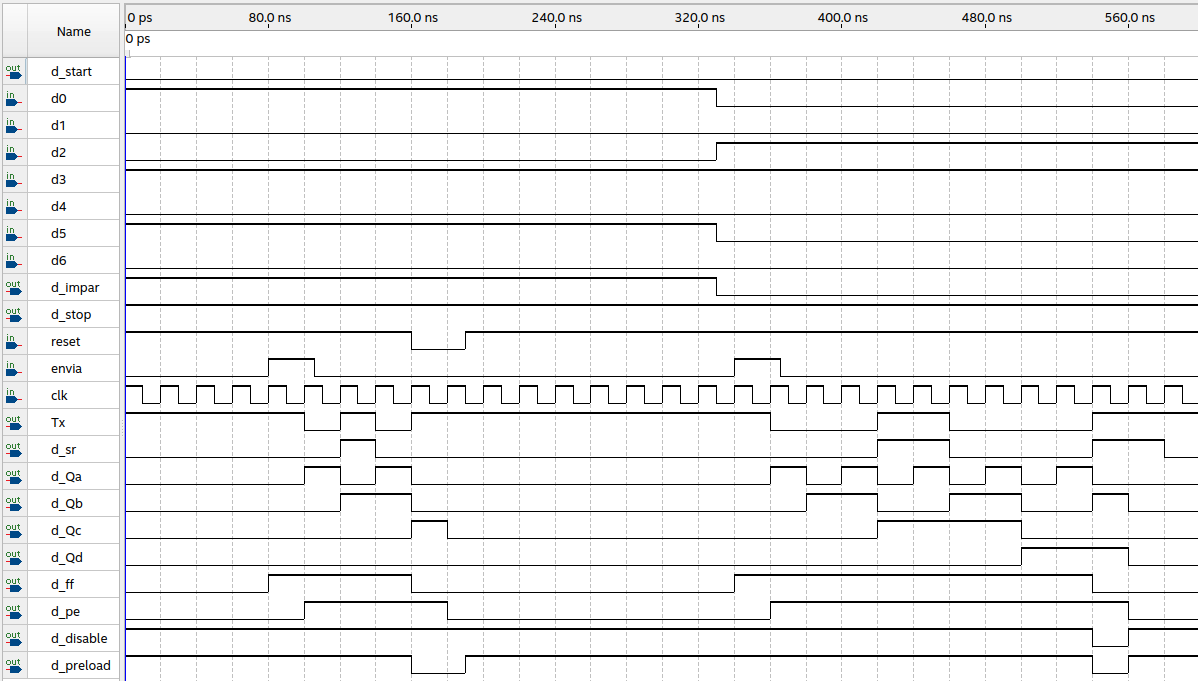
\includegraphics[width=\textwidth]{tc-2.png}
    \caption{Carta dos Tempos do segundo caso de teste}
    \label{fig:tc2}
\end{figure}

\newpage
\subsubsection{Terceiro Caso de Teste}
\label{ap:tc-3}
{\bf Descrição do Caso de Teste:} O sistema deve ser sensível à borda de subida do sinal \texttt{envia} e deve enviar apenas um pacote de dados e voltar para o estado de repouso, mesmo que o sinal \texttt{envia} ainda esteja alto. O sistema só podera enviar um novo pacote ao detectar uma nova borda de subida do sinal \texttt{envia}.

Esse caso de teste tem o objetivo de verificar se o sistema sairá do seu comportamento esperado caso o tempo de duração do sinal envia seja maior que o tempo de envio do pacote. Por exemplo, apertar o botão envia manualmente e receber um sinal de clock de um gerador de função com frequência da ordem de centenas de Hz.

\begin{figure}[!ht]
    \centering
    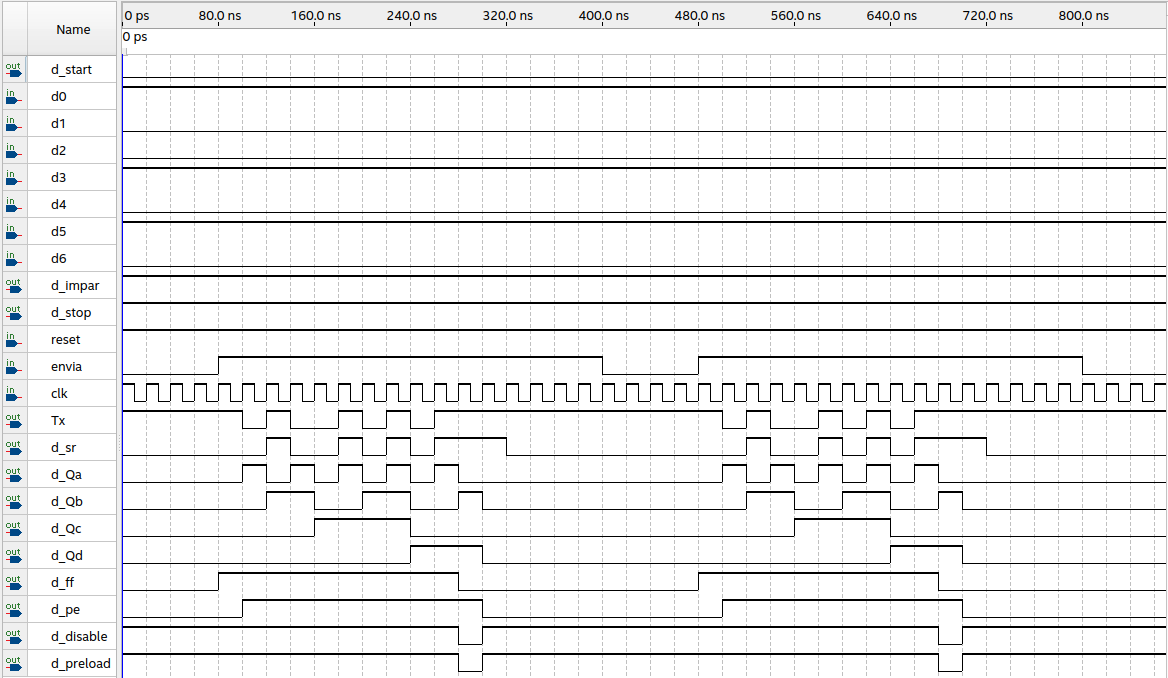
\includegraphics[width=\textwidth]{tc-3.png}
    \caption{Carta dos Tempos do terceiro caso de teste}
    \label{fig:tc3}
\end{figure}

\newpage
\subsubsection{Quarto Caso de Teste}
\label{ap:tc-4}
{\bf Descrição do Caso de Teste:} O sistema deve apresentar paridade ímpar. Isto é, o bit de paridade deve ter o nível lógico '1' se o número de níveis lógicos iguais a '1' nos bits de dados forem ímpar e '0' caso contrário.

Esse é um caso de teste base e tem o objetivo de verificar se o bit de paridade é calculado corretamente.

\begin{figure}[!ht]
    \centering
    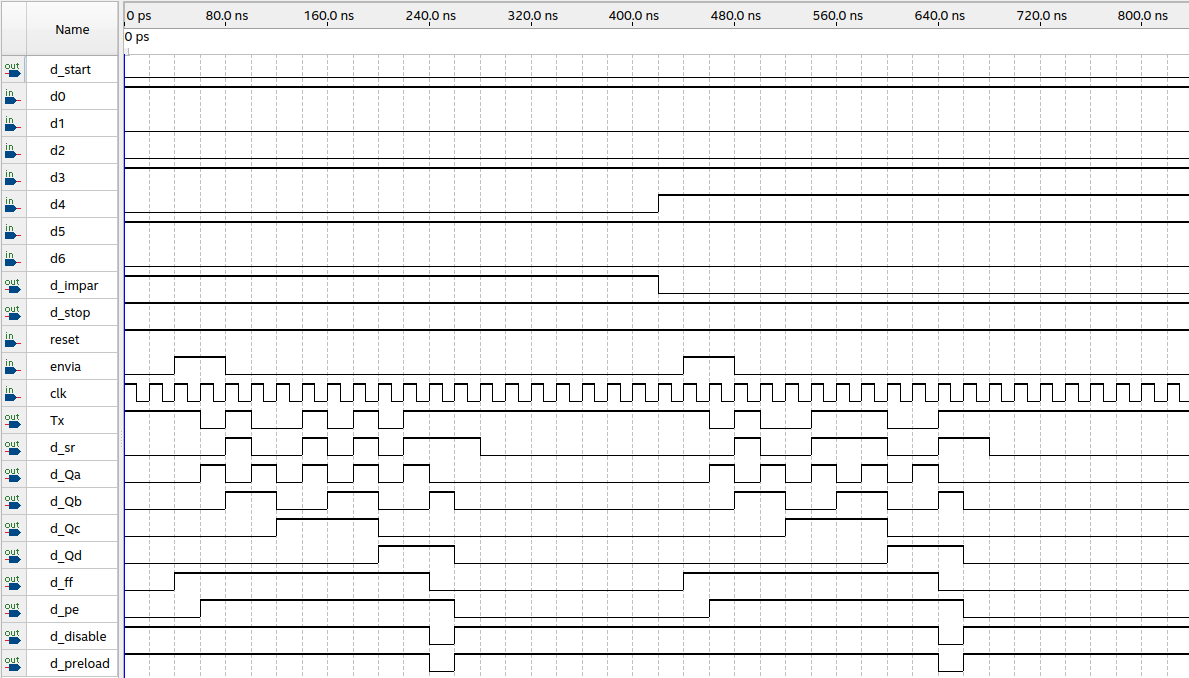
\includegraphics[width=\textwidth]{tc-4.png}
    \caption{Carta dos Tempos do quarto caso de teste}
    \label{fig:tc4}
\end{figure}



\newpage
\subsection{Tabela de Depuração}
\label{ap:tb-dep}

\begin{table}[!ht]
    \centering
    \caption{Tabela de depuração do envio de uma palavra genérica $d_6d_5d_4d_3d_2d_1d_0$}
    \label{tab:tb_testes_74163}
    \doubleRuleSep
    \begin{tabular}{*{14}{c}}
        \doubleTopRule
        \multicolumn{3}{c}{Entradas} & \multicolumn{9}{c}{Sinais de Depuração} & Saída\\
        \cmidrule(lr){1-3}\cmidrule(lr){4-12}\cmidrule(lr){13-13}
        clk & envia & reset & Qa & Qb & Qc & Qd & ff & pe & disable & preload & sr & Tx & *\\
        \midrule
        \csvreader[head to column names, late after line=\\]{tb_dep.csv}{}%
        {\csvcoli & \csvcolii & \csvcoliii & \csvcoliv & \csvcolv & \csvcolvi & \csvcolvii & \csvcolviii & \csvcolix & \csvcolx & \csvcolxi & \csvcolxii & \csvcolxiii & \csvcolxiv}%
        \doubleBottomRule
    \end{tabular}
\end{table}

$^1$ Detecção da borda de subida do sinal \texttt{envia}, carregamento dos dados paralelos (1 clock), sinal Tx continua em repouso; ff tem sinal '1' daqui até o clock 11 (11 clocks)

$^2$ Transmissão do \texttt{start bit}; pe tem sinal '1' daqui até o clock 12 (11 clocks)

$^3$ Transmissão do bit $d_0$

$^4$ Transmissão do bit $d_1$

$^5$ Transmissão do bit $d_2$

$^6$ Transmissão do bit $d_3$

$^7$ Transmissão do bit $d_4$

$^8$ Transmissão do bit $d_5$

$^9$ Transmissão do bit $d_6$

$^{10}$ Transmissão do bit de paridade

$^{11}$ Transmissão do primeiro \texttt{stop bit}; ff preicsa ter sinal '0' a partir deste clock até a próxima borda de subida do sinal \texttt{envia}; disable e preload precisam ter sinal '0' apenas neste clock

$^{12}$ Transmissão do segundo \texttt{stop bit}; pe preicsa ter sinal '0' a partir deste clock até o clock do próximo \texttt{start bit}

$^{13}$ Estado de repouso

$^{14}$ Reset

\newpage
\subsection{Mapa de Karnaugh do Circuito Controlador}
\label{ap:74163_karnaugh}

\begin{figure}[!ht]
    \centering
    \resizebox{0.5\textwidth}{!}{%
        \begin{karnaugh-map}[4][4][1][$Q_DQ_C$][$Q_BQ_A$]
            \minterms{3,7,10,11,14,15}
            \autoterms[0]
            \implicant{3}{11}
            \implicant{15}{10}
        \end{karnaugh-map}%
    }
\caption{Mapa de Karnaugh do Circuito Controlador do circuito com o contador 74LS163}
\label{fig:karnaugh_74163}
\end{figure}


% \bibliographystyle{plainnat}
% \bibliography{refs}

\horizonBackCover
\end{document}